\input{preamble}

\usepackage{booktabs}

\begin{document}

\setlist{noitemsep}  % Reduce space between list items (itemize, enumerate, etc.)
\onehalfspacing      % Use 1.5 spacing
% Use endnotes instead of footnotes - redefine \footnote command
%\renewcommand{\footnote}{\endnote}  % Endnotes instead of footnotes

\author{Rasmus M. Jensen \& Morten B. Krogh\thanks{\rm Jensen \& Krogh are both Master Students at Aarhus School of Business and Social Sciences, Aarhus University. We thank our suporvisor Stig Vinther Møller for making this project possible with passionate and inspirational guidance.}}

\title{\Large \bf Business Cycles and predictability of returns under habit formation\footnote{The code used for this paper is based upon \cite{Campbell1999}'s GAUSS code out code available at \url{https://github.com/MortenBKrogh/Habit-Models-Advanced-Asset-Pricing}. The code is written in MATLAB 2019b, and is only able to run on a Windows machine due to that \textit{quadlab} file.}}

\date{}              % No date for final submission

% Create title page with no page number

\maketitle
\thispagestyle{empty}

\bigskip

\centerline{\bf ABSTRACT}

\begin{doublespace}  % Double-space the abstract and don't indent it
  \noindent We recalibrate the model of \citet{Campbell1999} on up-to-date US-data and simulate 100.000 months of returns in order to examine whether the model is able to generate data that is predictable during recessions. In addition we provide results on the overall out-of-sample predictability of stock returns generated from an external habit model.
\end{doublespace}

\medskip

\noindent \textit{Keywords: Consumption-based asset pricing, Habit formation.} \\

\noindent JEL classification: G11, G12, G32

           
  

\clearpage

\section{Introduction} \label{sec:Introduction}

\begin{comment}
idé gør som Cochrane og Campbell 1999:
\begin{enumerate}
    \item Kalibrer modellen (Mikrofundament)
    \item Simulér variable og PD
    \item Lav Recesssionsdummy fra surplus consumption / consumption
    \item Cross-sectional regressions med dummies
    \item Kan man forecaste OoS returns under recession og ikke expansion <- theoretical
\end{enumerate}

\hline

\begin{enumerate}
    \item evidence for predictability in recessions is already established, however due to the fact that the state of the economy only is recession approximately 10\% of the time, we find it interesting to investigate the power of the model in expansions as well. 
    \item This investigation will be conducted relaying heavily upon \cite{Campbell1999} and using a regime switchin regression framework. 
    \item The recession dummy will be construted from the surplus consumption ration simple as follows
    \begin{align}
        rec_t & = \begin{cases} 1 & \text{, if } s_t < \Bar{s} \\
                              0 & \text{, if } s_t > \Bar{s} \end{cases}
    \end{align}
    
    and the regression equation below
    
    \begin{align}
        r_{t+h} & = \alpha + \beta_1 \times r_t + \underbrace{\beta_2 \times pd_t  \times I_{rec_t}}_{\text{recession indicator}} + \underbrace{\beta_3 \times pd_t \left(1 - I_{rec_t} \right)}_{\text{Expansion Indicator}} + \varepsilon_{t+h} 
    \end{align}
    
    skriv noget om hvad andre har fundet ud af, nævn stigs 2013 artikel ifm. bond return predictability og nævn andre campbel osv der finder unpredictability i returns.

\end{enumerate}




This paper investigates the Habit Formation model proposed by \cite{Campbell1999} ability to predict in expansions as well as the out-of-sample performance of the model. 
The history of Asset Pricing models have provided evidence of predictability in periods of economic downturn \colorbox{yellow}{\textbf{INDSÆT KILDER}}, however, there have been little evidence showing predictability in expansions. The ability to predict in expansions are a highly desired capability, due to the fact the economy historically is in the state of expansion more often than recession. In the \cite{Campbell1999} framework, recession is defined as period where surplus consumption is below steady-state, hence the models recession is not exactly equal to the definition of three quarters of negative GDP growth as we are used to...


\hline

We examine the \cite{Campbell1999} model of Habit formation in asset pricing. Investigating the models performance both in recessions, which multiple sources have provided evidence of predictability of returns, and in expansions where it has been the case to be more difficult to predict returns. 

We calibrate the model based on newer data than \cite{Campbell1999}, then we perform a simple regression with an indicator variable of recession and $(1-I_{rec}$ for expansions, this is done for the ability to distinguish between model performance in recessions as well as in expansions. 

A recession in the model is defined as when surplus consumption is below some given value, that is 

    \begin{align}
        I_{rec} & = \begin{cases} 1 & \text{, if } s_t < s_{rec} \\
                                  0 & \text{, if } s_t > s_{rec} 
                    \end{cases}
    \end{align}

in order to match the empirical amount of times the economy have been in recession according to \cite{USREC} in the period $1950 - 2018$ $\approx 13 \%$, the threshold $s_{rec}$ needs to take a value somewhere below $s_{bar}$, otherwise if $s_{bar}$ is used as threshold the economy of the model will be in recession approximately $37\%$ of the time, this three times more than the economy actually have been in the last 68 years, thus the need for lowering the threshold. The threshold value of the surplus consumption ratio is found by integrating over the stationary distribution of the surplus consumption ratio.




We show that the model of \citet{Campbell1999} is capable of generating returns consistent with the empirical findings of \citet{Henkel2011}. That is returns which inherits the properties that they are predicable in recession but unpredictable in expansions.\\

\citet{Henkel2011} found that the predictability of returns using popular measures such as the dividend yield diminishes in expansions while remaining of significance during recessionary periods. \\

We simulate an economy according to \cite{Campbell1999}, and re-calibrate the parameters of the model to an extended period spanning \textit{1950-2018} compared to \citep{Campbell1999}'s \textit{1950-1994}. In an attempt to incorporate relevant information of the Great Financial Crisis of 2008 in our calibration.




Predictability of asset prices in expansions is a desirable capability since the economy is in a state of expansion more often than recession. In the period $1950-2018$\footnote{According to \cite{USREC}} the economy has been in recession $13.41\%$ of the time, hence being able to predict asset prices in expansions would yield a higher profit for investors.
\end{comment}

%\begin{comment}
A corner area of the consumption based asset pricing is to incorporate habits in an agents preferences, \textit{Habit Formation}. The idea, initiated by \citet{Constantinides_1990}, assumes that marginal utility of consumption rely on consumption relative to stochastic habit process which is related to past consumption, thus utility is a function of both consumption and habits $u \left(C_t, X_t \right)$. This captures a fundamental psychological feature of human behavior, namely when income rises consumption only slowly adapts, thus being exposed to a stimulus again and again reduces the response. 

\citet{Campbell1999} considers a model with external habit, that is habit depends on aggregate consumption, and thus is unaffected by a single agents choices, this type of habit is also refereed to as \textit{>>catching up with the Joneses<<}. They specify the consumption utility function as a power function of differences $C_t - X_t$ and are able to match empirical features of the economy such as the excess return on stocks, the sharpratio and riskfree rate to mention a few. 

In this paper we follow \citet{Campbell1999} approach and are able to reproduce their results, then we re-calibrate the parameters of the model by extending the period spanning  $1950 \ -  \ 2018$, this includes the both the \textit{>>dot com bubble<<} in 2000 and the \textit{>>Great Financial Crisis<<} in 2007-2009, incorporating this period is an attempt to capture more recent and relevant information in the calibration. We define an indicator for recession to match the amount of times the economy has been in recession in the data period \textit{13.4\%}, and estimate both the ordinary asset pricing regression where we divide effects of predictability into recession- and expansion periods, besides this we also estimate a regime switching regression where the left hand side is conditioned upon the indicator. 
The results show that the model of \citet{Campbell1999} is capable of generating returns consistent with the empirical findings of \citet{Henkel2011}. That is returns which inherits the properties that they are predicable in recession but unpredictable in expansions.

%\end{comment}
\section{Data} \label{sec:Data}

\section{Model framework} \label{sec:Methodology}

The framework utilized is a direct application of the model by \citet{Campbell1999} in the following section a brief overview of the model and model dynamics are presented.\\
The model can be seen as an extension of the basic consumption-based asset pricing framework in that the standard CRRA-utility function is augmented with habit formation. 
\begin{align}
   U(C_t, X_t) = \mathbb{E} \sum _ {t = 0} ^{\infty} \delta ^ t \frac{\left( C_t - X_t\right)^{1-\gamma } - 1}{1-\gamma }
\end{align}
Where $X_t$ denotes the habit level, $\delta$ is the subjective discount factor  of the agents. \citet{Campbell1999} proposes that the entire economy can be summarized by the state variable capturing the relationship between consumption and habit - the \textit{surplus-consumption ratio} $S_t$.
\begin{align}
   S_t \equiv \frac{C_t - X_t}{C_t} \label{S_t_Process}
\end{align}
The surplus consumption ratio can thus be interpreted as the consumption level above above the habit level. This formulation ensures that the surplus consumption ratio does not go below 0, however as $X_t$. approaches $C_t$ the surplus consumption ratio converges to $0$, which indicates an extreme case where the risk aversion in the economy diverges, this result follows directly from the expression of the local curvature of the utility function.
\begin{align}
    \eta _t \equiv - \frac{C_t U_{cc}\left( C_t, X_t \right)}{U_{c} \left( C_t, X_t \right)} = \frac{\gamma}{S_t}
    \end{align}
However this result, while not well behaved in extreme cases, implies a convenient feature of this model, namely that the degree of risk aversion increases (decreases) as the surplus consumption ratio declines (increases). The economic interpretation is that as the growth of wealth and by extension consumption falls below the usual level, the risk aversion of the agents increases which is a well known trait of agent behavior and the driving forces behind this phenomena are studied more throughout in behavioral economics.\\
\newline
Also following \citet{Campbell1999} the law of motion of log surplus consumption ratio is defined as a heteroscedastic autoregressive model of order 1,
\begin{align}
    s_{t+1}^a  = \left( 1-\phi  \right)\Bar{s}+ \phi s_t ^ a + \lambda \left( s_t ^a  \right)\left( c_{t+1}^a - c_t^a - g\right) \label{ARHet}
\end{align}
where $\lambda(s_t^a)$ is a sensitivity function whose functional form will be further specified below and $\Bar{s},\phi, g$ are parameters either to be matched or calibrated. We note that around the steady state the rational agents all behave equivalent to one another, and the superscript \textit{a}, denoting aggregate measures can be dropped.
The last term of \eqref{ARHet} follows from the assumed functional form of consumption growth,
\begin{align}
    \Delta c_{t+1} = g + v_{t+1}, \qquad v_{t+1}\overset{\mathcal{IID}}{\sim}\mathcal{N}\left(0, \sigma^2 \right) \label{DConos}
\end{align}
hence,
\begin{align}
     c_{t+1} - c_t - g = v_{t+1}
\end{align}
\subsection{Stochastic discount factor/pricing kernel}
Starting from the utility function of the rational agent,
\begin{align*}
    U(C_t, X_t) = \mathbb{E} \sum _ {t = 0} ^{\infty} \delta ^ t \frac{\left( C_t - X_t\right)^{1-\gamma } - 1}{1-\gamma }
\end{align*}
the first order condition with respect to consumption,
\begin{align*}
    U_c \left( C_t, X_t \right) = \frac{\partial}{\partial C_t} U(C_t, X_t) & = \left( C_t - X_t\right)^{-\gamma}
\end{align*}
Substituting $X_t$ from \eqref{S_t_Process}:  $(-X_t = S_t)$,
\begin{align}
     U_c \left( C_t, X_t \right) = S_t ^{-\gamma} C_t ^{-\gamma}
\end{align}
The stochastic discount factor can then be expressed,
\begin{align}
    M_{t+1} & \equiv  \delta \frac{u_c\left( C_{t+1}, X_{t+1} \right)}{u_c\left( C_{t}, X_{t} \right)} \nonumber \\
    & = \delta \left( \frac{S_{t+1} C_{t+1}}{S_t C_t} \right) \label{SDF}
\end{align}
Collecting previous expressions in the system and plugging into \eqref{SDF},
\begin{equation}
M_{t+1}=\delta G^{-\gamma} e^{-\gamma\left(s_{t+1}-s_{t}+v_{t+1}\right)}=\delta G^{-\gamma} e^{\left.-\gamma(\phi-1)\left(s_{t}-s\right)+\left[1+\lambda\left(s_{t}\right)\right] v_{t+1}\right\}}
\end{equation}
Which can be viewed as the pricing kernel utilized in this paper, conditional moments of all variables of interest can be derived from this equation which is a function of the state $s_t$.

\subsection{Risk-free Rate}
In the framework by \citet{Campbell1999} the risk-free rate is assumed to be constant, this follows from the definition of the risk-free rate,
\begin{align}
    R_t^{f} \equiv \frac{1}{\mathbb{E}_t \left[ {M_{t+1}} \right]} \nonumber
\end{align}
using equation \eqref{SDF} yields the log risk-free rate,
\begin{align}
    r_t^{f} = -\ln \left(\delta \right) + \gamma g - \underset{A}{\underbrace{\gamma \left( 1-\phi \right)\left( s_t - \Bar{s} \right)}} - \underset{B}{\underbrace{\frac{\gamma ^2 \sigma ^2 }{2} \left( 1+ \lambda\left( s_t \right) \right)^2}} \label{RFR}
\end{align}
to make sure $R_t^f$ is constant \citet{Campbell1999} chooses the functional form of $\lambda\left( s_t \right)$ such that the effects of intertemporal substitution (\textit{A}) offsets the precautionary savings-term (\textit{B }).\\
\newline
In addition the functional form of $\lambda(s_t)$ is chosen to satisfy two additional conditions, the three conditions are then given:
\begin{enumerate}
    \item Risk-free rate constant through time
    \item Habit is predetermined at steady-state
    \item Habit is predetermined close to steady-state
\end{enumerate}
These conditions yields an expression for the steady-state surplus consumption ratio,
\begin{align}
    \Bar{S} = \sigma \sqrt{\frac{\gamma }{1-\phi}}
\end{align}
Implying a predetermined habit level in the steady-state. In addition the sensitivity function is then specified,
\begin{align}
    \lambda \left( s_t \right) = \begin{cases}
    {\frac{1}{\Bar{S}}\sqrt{1-2\left( s_t - \Bar{s} \right)}-1, \qquad &s_t \leq s_{\max}\\
    0, \qquad & s_t\geq s_{\max}}
    \end{cases}
\end{align}
where $S_\max$ is the solution to
\begin{align}
    0 & = {\frac{1}{\Bar{S}}\sqrt{1-2\left( s_{\max} - \Bar{s} \right)}-1}\\
    s_{\max} & = \Bar{s} + \frac{1}{2}\left( 1 - \Bar{S}^2\right)
\end{align}
Now substituting in these results into equation \eqref{RFR} yields a time-invariant risk-free rate as per construction.
\begin{equation}
r_{t}^{f}=-\ln (\delta)+\gamma g-\left(\frac{\gamma}{S}\right)^{2} \frac{\sigma^{2}}{2}=-\ln (\delta)+\gamma g-\frac{\gamma}{2}(1-\phi) \label{RFR1}
\end{equation}
Now to refine the framework one could implement a time-varying risk-free rate as suggested by \citet{Campbell1999} and implemented by \citet{Wachter2005}. A time-varying risk-free rate allows for the construction of term-structures as a function of the state variable, this suggests that by correct specification the term-structure is predictable using the surplus consumption ratio.\\
However \citet{Campbell1999} argues that that the risk-free rate in US-data exhibits limited variation furthermore extending the model with a time-varying risk-free rate has little to no effect on the results regarding the stock market, therefore the model specification used in this paper assumes a constant risk-free rate, consistent with the model in \citet{Campbell1999}.

\subsection{Pricing a Consumption Claim}
The actual pricing relations in this part while very simple analytically, are the most comprehensive part computational and numerical, this follows from the fact that the the price-dividend ratio as a function of state-variable $s_t$ are not observable and are thus solved on a grid using the Gauss-Legendre quadrature procedure for numerical integration. \\
\newline
To clarify economical procedure, we will utilize the basic pricing relation that is,
\begin{align}
    1 = \mathbb{E}_t \left [ M_{t+1}R_{t+1} \right] \nonumber \\
    R_{t+1} \equiv \frac{P_{t+1} + D_{t+1}}{P_t}
\end{align}
The functional $P_t/C_t(s_t)$ must then satisfy,
\begin{align}
    \frac{P_{t}}{C_{t}}\left(s_{t}\right)=E_{t}\left[M_{t+1} \frac{C_{t+1}}{C_{t}}\left[1+\frac{P_{t+1}}{C_{t+1}}\left(s_{t+1}\right)\right]\right] \label{PCRatio}
\end{align}
This functional is solved numerically over a grid of $s_t$ spanning $]0:s_max]$, to increase the precision of the estimation, the grid is a equally distributed linespace but augmented with more mass in the tails this allows the estimation to better capture non-linearities in the tail of the distribution of the price-consumption ratio. To determine P/C in-between grid-points we use an interpolation procedure.

The conditional expectation is then solved on a grid through the Gauss-Legendre procedure over the error term $v_t$.

\subsection{Pricing a Dividend Claim}
The dividend claim process is solved in the same manner as in the previous section however the IID log-normal process for dividend growth is constructed such that the innovations in the dividend growth $w_t$ and in consumption $v_t$ is correlated with magnitude $\rho$,
\begin{align}
    \Delta d_{t+1} = g + w_{t+1},\qquad w_t \overset{\mathcal{IID}}{\sim}\mathcal{N}\left(0,\sigma^2_w \right),\qquad \operatorname{corr}\left( w_t,\ v_t \right) = \rho
\end{align}
The functional price-dividend ratio is then calculated in the same manner as \eqref{PCRatio}
\begin{align}
    \frac{P_{t}}{D_{t}}\left(s_{t}\right)=E_{t}\left[M_{t+1} \frac{D_{t+1}}{D_{t}}\left[1+\frac{P_{t+1}}{D_{t+1}}\left(s_{t+1}\right)\right]\right] \label{pd_ratio}
\end{align}
It is worth noting that \citet{Campbell1999} actually recommends that the relationship between dividend growth and consumption growth should in fact be co-integrated rather than correlated, however we will be closing the model with a correlational relationship rather than the co-integrational relation proposed\footnote{\textsc{MatLab} code are available at GitHub, and are modified from the code presented by \citet{Costa2009}}. 

\subsection{Calibration of the model parameters}
For model calibration we will rely on CRSP-data retrieved from the WRDS-database. The sampling period utilized spans 1950-2018 and samples 90 day T-bill returns and inflation rate \textit{Annual}, CRSP-Market return index\footnote{Index spanning the 2 stock exhanges NYSE/AMEX} \textit{Monthly and annual}, and \textit{FRED} personal consumption data non-durables \textit{Quarterly}.  


We will utilize the analytical results presented by \citet{Campbell1999} and \citet{StigVinter2010}

To estimate the unconditional mean of the consumption growth, $g$, in the model we apply the expectations operator to equation \eqref{DConos},
\begin{align}
    \mathbb{E}\left[ \Delta c_{t+1} \right] &=  \mathbb{E}\left[ g + v_{t+1} \right],\qquad v_t\overset{IID}{\sim}\mathcal{N}\left(0,\sigma\right), \qquad \forall t\nonumber \\
    & = g
\end{align}
hence a consistent estimate of the true unconditional mean is given as the sample mean of consumption growth. From this result follows by extension that the unconditional standard deviation is given by $\sigma$ while the consistent estimate is simply the sample standard deviation of the consumption growth, the same result applies to dividend growth.

To determine the correlation between dividend growth and consumption ratio ${\operatorname{corr}(w_t, v_t)}$ or $\rho$ we follow the argumentation of \citet{Campbell1999} the correlation between dividend growth and consumption growth are especially tricky to calibrate as it is very non-robust to horizon changes, hence we fix the correlation to the level chosen by \citet{Campbell1999}, they use $\rho = 0.2$ but notes that with different horizons the value lies between (0.05-0.25).\\
To estimate the true autocorrelation-coefficient we use the first order sample autocorrelation function of the dividend-price ratio, i.e,
\begin{align}
      d_t - p_t = \alpha + \phi \left( d_{t-1}-p_{t-1} \right)+\varepsilon_t
\end{align}
These dynamics of the dividend yield are true only if the best forecast of future dividend yield can be retrieved from an AR(1) model, that this holds true can be seen from equation \eqref{pd_ratio}, stating the the price-dividend ratio is a functional only of the state variable, hence inheriting the dynamics of only one state, the surplus consumption ratio. This hold true for all $t$ thus the effects of $s_t$ on $d_{t+1}-p_{t+1}$, can be retrieved using the information contained in $d_t-p_t$.\\
The local utility curvature, $\gamma$, in the model is not calibrated as per say, instead we rely on existiing literature such as \citet{Campbell1999} and fixes $\gamma = 2$.
\\
\newline
The subjective discount factor is chosen as to match the risk-free rate as reported in the CRSP-data. 
Recalling equation \eqref{RFR1} allows for a closed form solution for subjective discount factor given an arbitrary calibration of the risk-free rate, the local utility curvature, the persistence coefficient and the growth rate of dividends/consumption,
\begin{align}
    \delta = \exp{\left( \gamma g - \frac{1}{2} \left( \left(1-\phi\right)\gamma  \right) - r^{f} \right)}
\end{align}
that is when the model has been calibrated with all of the estimates above, there exists one unique solution to the $\delta$ parameter.
\section{Analysis} \label{sec:Analysis}

\subsubsection{Calibrated Model}

\begin{table}[H]
\begin{adjustbox}{max width=\textwidth}
\begin{threeparttable}[b]
\caption{Parameters of the model}
\label{tab:ModelCalib}
\begin{tabular}{@{}lllcc@{}}
\toprule
 & Parameter                              & Notation         & Calibration & \citet{Campbell1999}\\ \midrule 
\multicolumn{5}{l}{\textit{Calibrated}}                                    \\
 & Mean consumption growth                & $g$              & $0.0134$  & $0.0189$\\
 & Standard deviation of $\Delta c_t$     & $\sigma$         & $0.0152$  & $0.0150$\\
 & Standard deviation of $\Delta d_t$     & $\sigma_w$       & $0.1256$  & $0.1120$\\
 & Log risk-free rate                     & $r^f$            & $0.0109$  & $0.0094$\\
 & Persistence parameter                  & $\phi$           & $0.9008$  & $0.8700$\\
 \multicolumn{5}{l}{\textit{Assumed}}                                      \\
 & Coefficient of Risk Aversion           & $\gamma$         & $2.0000$  & $2.0000$\\
 & Correlation dividends/consumption      & $\rho$           & $0.2000$  & $0.2000$\\
\multicolumn{5}{l}{\textit{Implied}}                                       \\
 & Subjective discount factor             & $\delta$         & $0.9156$  & $0.8900$\\
 & Steady-state surplus consumption ratio & $\Bar{S}$        & $0.0666$  & $0.5700$\\
 & Maximum surplus consumption ratio      & $S_{\text{max}}$ & $0.1096$  & $0.0940$\\ \bottomrule
\end{tabular}
\begin{tablenotes}
\footnotesize{\item [1] All relevant parameters are annualized
              \item [2] Calibrated parameters are estimated from data, assumed are chosen arbitrarily on the grounds of existing literature, while implied parameters are calculated from the calibrated/assumed parameters.}
\end{tablenotes}
\end{threeparttable}
\end{adjustbox}
\end{table}


Compared to the calibration of \citet{Campbell1999}, our calibration suggests a higher persistence parameter, higher volatility of dividend growth and lower consumption growth, the implied surplus consumption parameters suggests a slightly higher overall surplus consumption. The differences likely stems from the extra 20 years of calibration data. \\

\subsection{Simulation}
From the calibrated model we simulate a chain of 100.000 monthly draws from the economy yielding 8.332 years of simulated time-series. We find in addition to the series that the procedure is extremely sensitive to the distribution of grid points. We use 10 equally distributed grid-points and an additional 6 just below $s_max$.

\begin{table}[H]
\centering
\caption{Simulated Moments}
\label{tab:simmom}
\begin{tabular}{@{}lllll@{}}
\toprule
Statistic                                               & \makecell{Consumption \\ Claim} & \makecell{Dividend \\ Claim} & \makecell{CC99-Calibration \\ Consumption Claim} & \makecell{CC99-Calibration\\ Dividend Claim} \\ \midrule
$\mathbb{E}\left(\Delta c \right)$                      &0.013504&0.011661&0.019024&0.017369\\
$\sigma\left(\Delta c \right)$                          &0.01243&0.10257&0.012268&0.09147\\
$\mathbb{E}r^f$                                         &0.010881&0.010881&0.0094&0.0094\\
$\mathbb{E}\left(r-f^f\right)/\sigma\left(r-r^f\right)$ &0.37625&0.23074& 0.43644                                       &         0.31764                            \\
$\mathbb{E}\left(R-R^f\right)/\sigma\left(R-R^f\right)$ & 0.4173   & 0.31102               &  0.4761                                      &      0.389                               \\
$\mathbb{E}\left(r-r^f\right)$                          &  0.048783                 &      0.045342          &         0.067377                               &        0.06472                             \\
$\sigma\left(r-r^f\right)$                              &     0.12965              &       0.19651           &   0.15438                                       &                  0.19651                     \\
$\mathbb{E}\left(p-c\right)$                          &     3.1123                &      3.157            &         2.8926                                 &             2.9161                          \\
$\sigma\left(p-c\right)$                              &       0.26201            &      0.28973          &   0.27676                                     & 0.29361                                    \\ \bottomrule
\end{tabular}
\end{table}



Allowing us to infer about the predictability of excess stock returns, during times of simulated crisis. 
\newline
\\
Based on NCER-recession data, we find that the US economy was in recession approximately 13.4\% of the period spanning January 1950 until December 2018.  In the model a recession implies that present consumption in low relative to previous periods consumption, that is the value of $s_t$ is lower than the steady state value of surplus consumption $\Bar{s}$ - integrating over the density of $s_t$ yields that the simulated economy is in recession during 37\% of all observations, which indicates that $\Bar{s}$ might be misspecified. To correct $\Bar{s}$ we match the empirical business cycle behavior by numerical optimization of the $s_t$ density, such that the empirical and simulated economy is in recession roughly the same amount. The $\Bar{s}$-value matching the empirical business cycle, throughout denoted $\Bar{s}_{rec}$ \textit{or} ($\Bar{S}_{rec}$), is found to be $-3.18$ ($0.0415$). One additional recessions specification we denote as $\bar{s}_{2,rec}$ is chosen as to capture only the most extreme non-linearity of the relationship between surplus consumption and expected returns as presented in figure \ref{fig:SPCPD-a}.

\begin{table}[H] 
\centering
\caption{Business Cycle, Simulated and historic}
\label{tab:BC}
\begin{tabular}{@{\hspace{8mm}}ll@{\hspace{5mm}}ccc@{}}
\toprule
                       & \multicolumn{3}{c}{\textit{Simulated}} & \textit{Historic}  \\ \midrule
                                          & $\Bar{S}$       & $\Bar{S}_{REC}$ & $\Bar{S}_{2,REC}$&    \\ \cmidrule(l){2-4} 
        \textit{Value}                        & 0.067 & 0.042& 0.02 &              \\
Recession,                                      \% &36.92 & 13.41 &2.83  & 13.41\\ \bottomrule
\end{tabular}
\end{table}




\begin{figure}[H]
    \centering
    \caption{Distribution of simulated $s_t$ chain}
    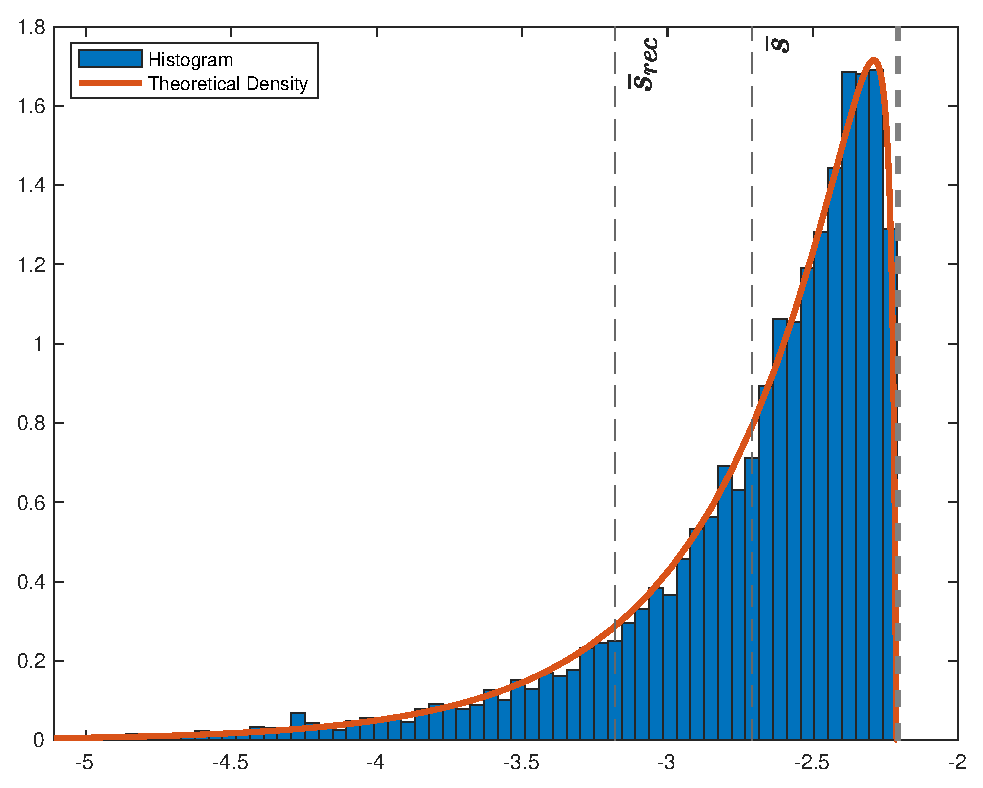
\includegraphics[width=\textwidth]{Figures/DistributionS_t.eps}
    \label{fig:DistriSt}
\end{figure}
From the constructed surplus consumption threshold $\Bar{s}_{rec}$ for recession, we construct an indicator dummy for recessions. Such that $I_{rec} = 1$ \textit{iff}. $\Bar{s}_{rec} > s_t$ and $I_{rec}=0$ otherwise.

Having simulated an economy based upon habit formation, and justified our choice of recession periods of the simulated series, we are able to test the proposed hypothesis:
\begin{enumerate}
    \item Is the model of \citet{Campbell1999} able to generate returns with the following two properties
    \begin{enumerate}
        \item Returns are predictable by the price/consumption- or the price/dividend-ratio under recessionary periods?
        \item Returns are unpredictable by the price/consumption- or the price/dividend-ratio under expansionary periods?
    \end{enumerate}
\end{enumerate}
Examining the expected returns as a function of the surplus consumption ratio, as in figure \ref{fig:SPCPD-a}. The model reveals a somewhat linear relationship for high values of the surplus consumption, the relationship however is much more steep and nonlinear when $S_t$ approaches ${S}_{REC}$, the goal is then to exploit this fact when predicting returns.


\begin{comment}
\begin{figure}[H]
    \centering
    \caption{Expected returns as a function of $S_t$}
    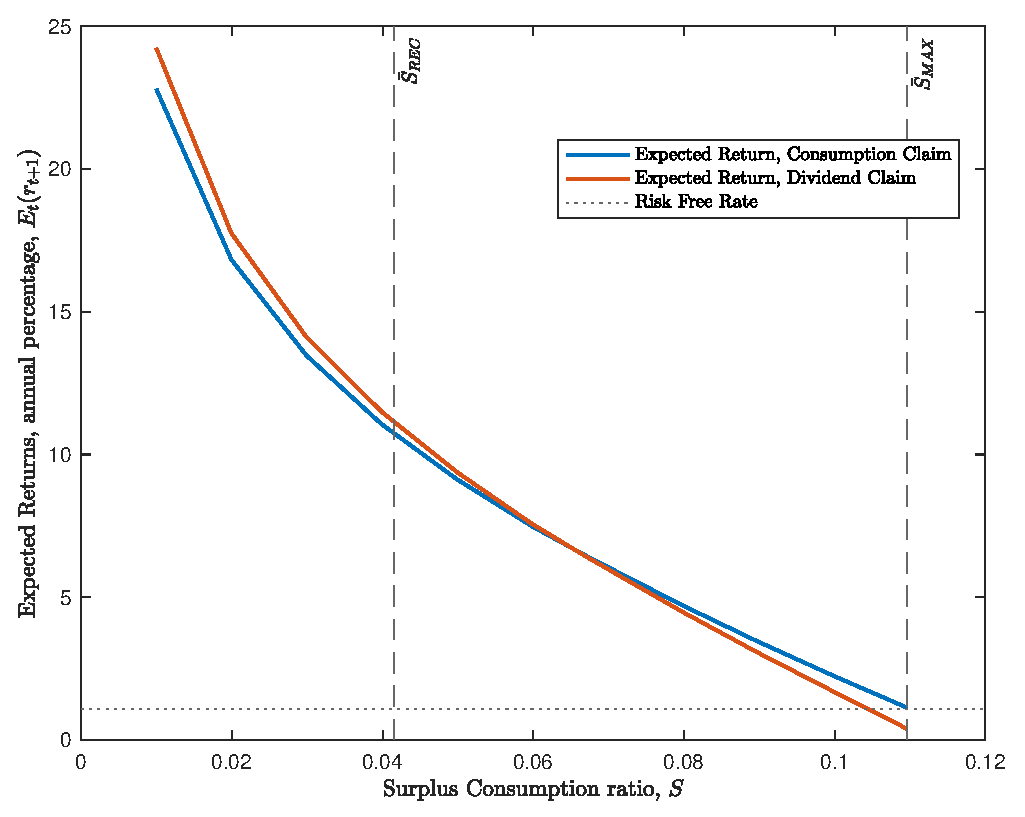
\includegraphics{Figures/ErPCPD.eps}
    \label{fig:ErPCPD}
\end{figure}
\end{comment}


\begin{figure}[H]
\centering
\caption{Functionals of surplus consumption ratio}
    \label{fig:SPCPD}
\subfigure[Expected returns as a function of $S_t$]{\label{fig:SPCPD-a}
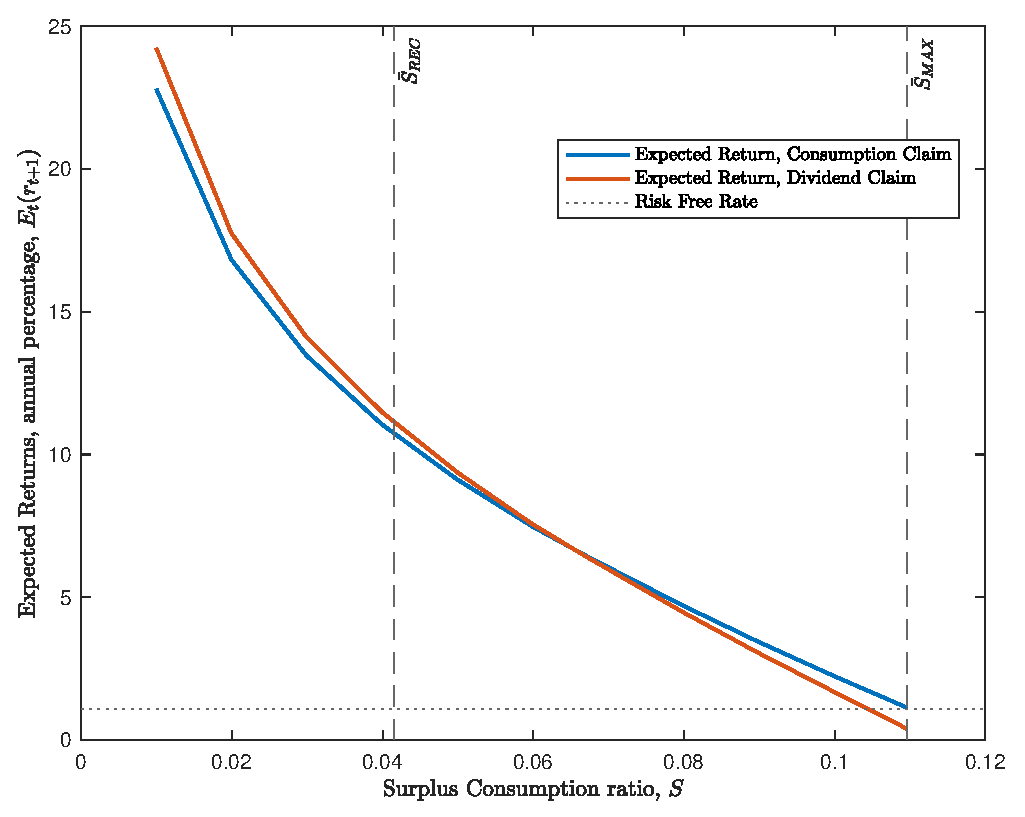
\includegraphics[width=0.45\textwidth]{Figures/ErPCPD.eps}} ~
\subfigure[$P/C$, $P/D$ as a function of $S_t$]{
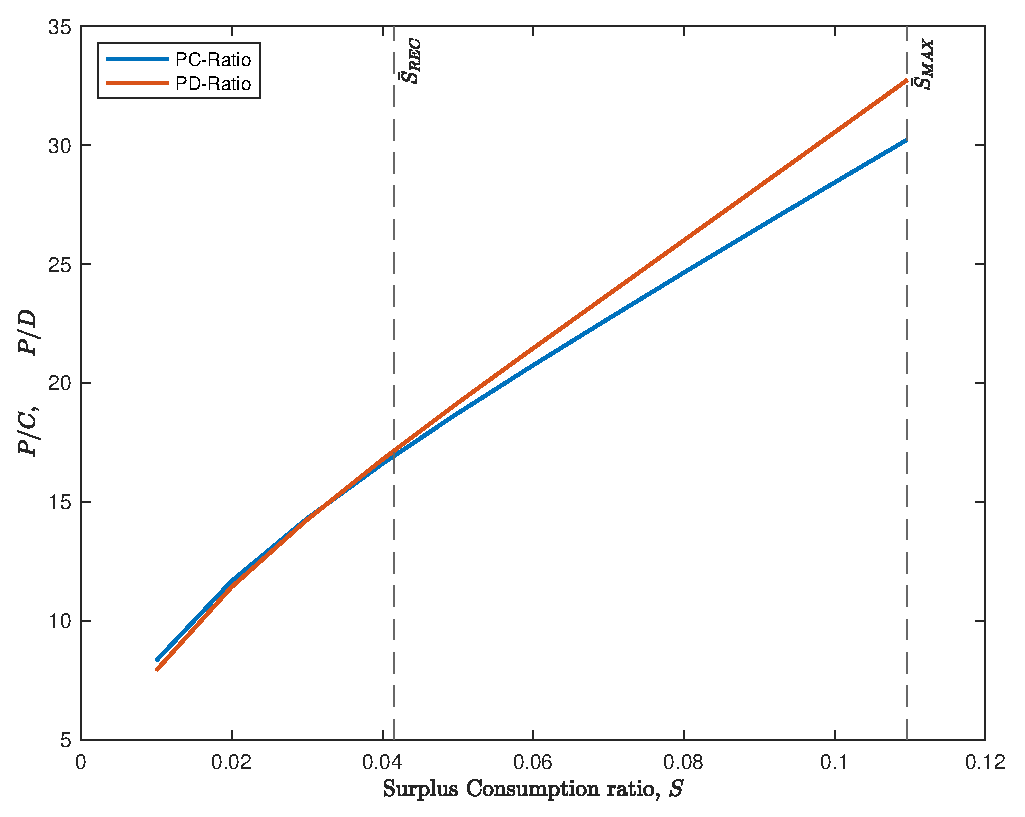
\includegraphics[width=0.45\textwidth]{Figures/PC_PD_Ratio.eps}}
\end{figure}

From the functionals of surplus consumption ratio reported in \ref{fig:SPCPD}, some basic predictions can be made. We see that when surplus consumption is low, that is in recessionary times, expected returns increases, the intuition is that when times are bad, as consumption falls relative to habit levels, the risk aversion increases, people wants a higher level of compensation per unit of risk - the risk premium rises - note that this must hold true for all levels of $S$ as the risk-free rate is fixed in the model.  


\subsection{Results}
First we estimate the following regressions:
\begin{align*}
     r_{t+1} - r^{f} &= \alpha + \beta_{REC} \left( p_t - c_t \right) * I_{t,REC} + \beta_{EXP} \left( p_t - c_t \right) * \left(1 - I_{t,REC}\right)  + \varepsilon_{t+1}\\
      r_{t+1} - r^{f} &= \alpha + \beta_{REC} \left( p_t - d_t \right) * I_{t,REC} + \beta_{EXP} \left( p_t - d_t \right) * \left(1 - I_{t,REC}\right)  + \varepsilon_{t+1}\\
      r_{t+1} - r^{f} &= \left(\alpha_{REC} + \beta_{REC} \left(p_t - c_t\right)\right)*I_{REC} + \left(1-I_{REC}\right) \left( \alpha_{EXP} + \beta_{EXP}\left(p_t - c_t \right) \right) + \varepsilon_{t+1}\\
r_{t+1} - r^{f} &= \left(\alpha_{REC} + \beta_{REC} \left(p_t - d_t\right)\right)*I_{REC} + \left(1-I_{REC}\right) \left( \alpha_{EXP} + \beta_{EXP}\left(p_t - d_t \right) \right) + \varepsilon_{t+1}      
\end{align*}
That is we use the recession indicator to infer the influence of the predictors in respectively recessions and expansions.\\
As a benchmark we run two additional regressions given:
\begin{align*}
     r_{t+1} - r^{f} &= \alpha + \beta \left( p_t - c_t \right)  + \varepsilon_{t+1}\\
      r_{t+1} - r^{f} &= \alpha + \beta \left( p_t - d_t \right) + \varepsilon_{t+1}
\end{align*}
Figure \ref{tab:regress1} reports results of the four regressions. The desired property of separability of business cycles does not get a lot of support from this exact result. We see no increase in $R^2$, we find strong statistical evidence supporting rejection of the null-hypothesis for all estimates in all four regressions, this is however to be expected as the sample size of 8331 observations is quite large, it is well established that as the sample size increases the asymptotic variance of the OLS-estimate decreases and thus significance is inevitable as the sample size becomes quite large.
\begin{table}[H]
\centering   
  \caption{Regressions, $\Bar{S}_{REC} = 0.041542$}           
  \label{tab:regress1}     
  \begin{threeparttable}
\begin{tabular}{@{\hspace{5pt}}l@{\hspace{5pt}}cccccc} 
\toprule 
 & \multicolumn{6}{c}{\textit{Dependent variable:}} \\ 
 & \multicolumn{6}{c}{$\left(r_{t+1}-r^f\right)$} \\ 
 \cmidrule(rr){2-7}
 & (1) & (2) & (3) & (4) & (5) & (6) \\ 
\midrule  
\\[-2.1ex] $\left( p_t - c_t \right)_{REC}$ &-0.169& &0.03228 & & &\\ 
  & (0.012) & &(0.0023) & & & \\ 
 \addlinespace 
  $\left( p_t - c_t \right)_{EXP}$ &-0.1641  &    & &-0.02975 & &  \\ 
  & (0.0098) & & &(0.0019) & & \\ 
 \addlinespace 
  $\left( p_t - d_t \right)_{REC}$ & &-0.1719& & & 0.03658  &   \\ 
                                   & &  (0.016) & & & (0.0031) &    \\ 
 \addlinespace 
  $\left( p_t - d_t \right)_{EXP}$ & &   -0.1668& & & &-0.03338 \\ 
                                   & &  (0.012) & & & &(0.0024) \\ 
 \addlinespace 
 Constant &0.5611 &0.5736&0.03789 &0.1313 &0.03305 &0.1395 \\ 
          &(0.032) &(0.041)&(0.0013)&(0.0059)&(0.0021)&(0.0077) \\ 
 \addlinespace 
\midrule  
Observations & 8331 & 8331&8331 & 8331&8331&8331\\
R$^{2}$ &0.094 & 0.053&0.047&0.062&0.026&0.035 \\ 
Residual Std. Error &0.015 & 0.037&0.016&0.016&0.038&0.037 \\ 
\bottomrule 
\end{tabular} 
\begin{tablenotes}
\footnotesize{
\item[1] Brackets below estimates contains Newey-West corrected standard errors. 
\item[2] Regressions on 8331 years of simulated data.
\item[3] EXP (REC) denotes expansion (recession)
}
\end{tablenotes}
\end{threeparttable}
\end{table} 


However from figure \ref{fig:ErPCPD} we see that the most extreme effect of $S_t$ on expected returns kicks in at an estimated $0.02$, based on this fact we run additional regressions with the same specification as above, where we respecify $\Bar{S}_{REC}=0.02$, the output of which is reported in table \ref{tab:regress2}. This specification of $\Bar{S}_{REC}$ implies that the simulated economy is in recession approximately 2.8\% of the time.

\begin{table}[H]
\centering   
  \caption{Benchmark regressions}           
  \label{tab:regress1}     
  \begin{threeparttable}
\begin{tabular}{@{\hspace{5pt}}l@{\hspace{15pt}}c@{\hspace{5pt}}c} 
\toprule 
 & \multicolumn{2}{c}{\textit{Dependent variable:}} \\ 
 & \multicolumn{2}{c}{$\left(r_{t+1}-r^f\right)$} \\ 
 \cmidrule(rr){2-3}
 & (1) & (2)\\ 
\midrule  
\\[-2.1ex] $ p_t - c_t $ &-0.1516&\\ 
  & (0.0071) &  \\ 
 \addlinespace 
  $p_t - d_t $ & &   -0.137 \\ 
               & &  (0.0064) \\ 
 \addlinespace 
 Constant &0.5206 &0.4814\\ 
          &(0.023) &(0.021) \\ 
 \addlinespace 
\midrule  
Observations & 8331 & 8331\\
R$^{2}$ &0.094 & 0.094 \\ 
Residual Std. Error &0.015 & 0.015 \\ 
\bottomrule 
\end{tabular} 
\begin{tablenotes}
\footnotesize{
\item[1] Brackets below estimates contains Newey-West corrected standard errors. 
\item[2] Regressions on 8331 years of simulated data.
\item[3] EXP (REC) denotes expansion (recession)
}
\end{tablenotes}
\end{threeparttable}
\end{table} 


\begin{table}[H]
\centering   
  \caption{Regressions}           
  \label{tab:regress2}     
  \begin{threeparttable}
\begin{tabular}{@{\hspace{5pt}}l@{\hspace{5pt}}cccccc} 
\toprule 
 & \multicolumn{6}{c}{\textit{Dependent variable:}} \\ 
 & \multicolumn{6}{c}{$\left(r_{t+1}-r^f\right)$} \\ 
 \cmidrule(rr){2-7}
 & (1) & (2) & (3) & (4) & (5) & (6) \\ 
\midrule  
\\[-2.1ex] $\left( p_t - c_t \right)_{REC}$ &-0.1353& &0.06422 & & &\\ 
  & (0.013) & &(0.0056) & & & \\ 
 \addlinespace 
  $\left( p_t - c_t \right)_{EXP}$ &-0.1439  &     &-0.05878 & &  \\ 
  & (0.0081) & &(0.0037) & & \\ 
 \addlinespace 
  $\left( p_t - d_t \right)_{REC}$ & &-0.1205& & & & 0.06511  &   \\ 
                                   & &  (0.012) & & & & (0.0057) &    \\ 
 \addlinespace 
  $\left( p_t - d_t \right)_{EXP}$ & &   -0.1297& & & & &-0.05811 \\ 
                                   & &  (0.0073) & & & & &(0.0036) \\ 
 \addlinespace 
 Constant &0.4959 &0.4576&0.0441 &0.2274 &0.04412 &0.2281 \\ 
          &(0.026) &(0.024)&(0.0014)&(0.012)&(0.0014)&(0.012) \\ 
 \addlinespace 
\midrule  
Observations & 8331 & 8331& 8331&8331&8331\\
R$^{2}$ &0.094 & 0.094&0.039&0.072&0.039&0.074 \\ 
Residual Std. Error &0.015 & 0.015&0.016&0.016&0.016&0.016 \\ 
\bottomrule 
\end{tabular} 
\begin{tablenotes}
\footnotesize{
\item[1] Brackets below estimates contains Newey-West corrected standard errors. 
\item[2] Regressions on 8331 years of simulated data.
\item[3] EXP (REC) denotes expansion (recession)
}
\end{tablenotes}
\end{threeparttable}
\end{table} 




Instead we run a regime-switching linear regression with observable states, remember that from the simulation we obtained the surplus consumption ratio as an observable. In real data one would have to rely on latent state regressions such as a \textit{hidden Markov model}, to determine the latent state as a function of $s_t$.\\
However we have the simulated series and are able to run the regression straightforward. We run four regressions again with excess stock return as the regressand:

\begin{align*}
    \left(r_{t+1} - r^{f}\right) I_{t+1,REC} &=  \alpha + \beta \left( p_t - c_t \right) I_{REC,t} + \varepsilon_{t+1}\\
    \left(r_{t+1} - r^{f}\right)I_{t+1,REC} &=  \alpha + \beta \left( p_t - d_t \right) I_{REC,t} + \varepsilon_{t+1}\\
    \left(r_{t+1} - r^{f}\right)I_{t+1,EXP} &=  \alpha + \beta \left( p_t - c_t \right) \left( 1- I_{REC,t}\right)  + \varepsilon_{t+1}\\
    \left(r_{t+1} - r^{f}\right)I_{t+1,EXP} &=  \alpha + \beta \left( p_t - d_t \right) \left( 1- I_{REC,t}\right) x+ \varepsilon_{t+1}
\end{align*}

The results of the four regressions are reported in table \ref{tab:RSregress}, the results are quite interesting. Examining the results reveals that with a regime switching approach as opposed to the previous single state regression, we are able to split the effects of business cycles on the predictability of stock returns. Notice how the coefficients indicating the effects of respectively P/C and P/D ratios on excess returns have switched signs in recession periods, while the constant effect is negative during recessions, indicating the base effect of being in a recession on excess returns is negative. However while not intuitively inappropriate in this context it have to be noted that expected returns are restricted to be positive in this model, therefore mandating that the size of the log P/C and log P/D-ratios must be large enough to offset the negative constant. This restriction is not particular restrictive as the log price consumption-ratio and equivalent log price dividend ratio is seldom below 2, see the simulated chains of log P/C and log P/D in figure \ref{fig:PCPD} in appendix.\\

Another result worth noting is one that provides evidence in favor of both of our hypothesis, that is the estimated coefficient of determination is much higher in the recession periods reaching 7\% when predicting excess returns using the price-consumption-ratio, than it is in expansionary periods reaching just barely .2\%, using the price-dividend-ratio as the predictor yields a smaller $R^2$ this is to be expected, as the price-dividend is by construction a noisier mapping of the price-consumption-ratio dynamics, containing not only the shock to consumption growth $\sigma$ but also the shock to dividend growth $\sigma_w$.\\

Now in real data it is not plausible to condition the regressand on a future variable like we do with the recession indicator. The reason why it is still not completely unreasonable is the high persistence of $s_t$, remember that $s_t$ is driven by the highly persistent growth rate of consumption, estimating the persistence in our simulation yields an autocorrelation coefficient of $0.9972$.\\
In real data it would be more reasonable to estimate a transition probability matrix to forecast the underlying business cycle chain, and condition on the recession forecast. Recession forecasts, however, are notoriously unreliable, comtaminating the estimates with very high levels of uncertainty.


\begin{table}[H]
\centering   
  \caption{Regime Switching Regression}           
  \label{tab:RSregress}     
  \begin{threeparttable}
\begin{tabular}{@{\hspace{5pt}}l@{\hspace{5pt}}cccc} 
\toprule 
 & \multicolumn{4}{c}{\textit{Dependent variable:}} \\ 
 & \multicolumn{2}{c}{$\left(r_{t+1}-r^f\right)_{REC}$} & \multicolumn{2}{c}{$\left(r_{t+1}-r^f\right)_{EXP}$} \\ 
 \cmidrule(rr){2-5}
 & (1)   &   (2) & (3) & (4) \\ 
\midrule  
\\[-2.1ex] $ p_t - c_t $ & 0.001174&  &-0.0003139   & \\ 
  & (9.4e-05) & &(3.6e-05) & \\ 
 \addlinespace 
 $p_t - d_t$ &  & 0.001168 & &-0.000323 \\
 & & (9.4e-05) & &(3.523e-05) \\
 \addlinespace 
 Constant &-0.0005367 &-0.0005311 &0.00537 &0.005429 \\ 
  &(2.3e-05) &(2.3e-05) &(0.00018) &(0.00018) \\ 
 \addlinespace 
\midrule  
Observations & 99999 & 99999 & 99999 &99999\\ 
R$^{2}$ &0.009 & 0.0089 & 0.00036 &0.00039\\ 
Residual Std. Error &0.00045 & 0.00045 &0.001 & 0.001  \\ 
\bottomrule 
\end{tabular} 
\begin{tablenotes}
\footnotesize{
\item[1] Brackets below estimates contains \citet{NW87} corrected standard errors. 
\item[2] Regressions on 99999 months of simulated data.
\item[3] EXP (REC) denotes expansion (recession)
}
\end{tablenotes}
\end{threeparttable}
\end{table} 



\begin{comment}
\begin{table}[H]
\centering
\caption{Simulated Moments}
\label{tab:MMoomme}
\begin{tabular}{@{}llllllllll@{}}
\toprule 
 & $\mathbb{E}\Delta d$ & $\sigma_{\Delta d}$ & $\mathbb{E}r^f$ & $\mathbb{E}r^m/\sigma _{r^m}$ & $\mathbb{E}R^m/\sigma _{R^m}$ & $\mathbb{E}r^m$ & $\sigma_{r^m}$ & $\mathbb{E}d-p$ & $\sigma_{d-p}$  \\ 
\midrule 
\multicolumn{10}{l}{$P/D$}\\
 &0.011661&0.10257& 0.010881 & 0.19839 & 0.27412 & 0.034063 & 0.1717 & 3.4246 & 0.21183 \\ 
\multicolumn{10}{l}{$P/C$}\\
 &0.013504&0.01243& 0.010881 & 0.38534 & 0.42038 & 0.037242 & 0.096645 & 3.3797 & 0.1864 \\ 
\bottomrule 
\end{tabular}

\end{table}



\begin{table}[H]
\centering
\caption{Data Properties}
\label{tab:Data_props}
\begin{tabular}{@{}l@{\hspace{1.5cm}}l@{\hspace{1.5cm}}l@{}}
\toprule
 & \textit{Simulated} & \textit{Historic} \\ \midrule
$\mathbb{E}\left[r_t- r^f_t\right]$& $0.0373$           & $0.0927$          \\
$\sigma\left(r_t - r^f_t  \right)$ & $0.0962$           & $0.1670$          \\
$\mathbb{E}\left[r_t- r^f_t\right] / \sigma\left(r_t - r^f_t,\right)$ & $0.3877$ & $0.5548$  \\ \bottomrule
\end{tabular}
\end{table}
\end{comment}

\section{Conclusion} \label{sec:Conclusion}
We have shown how the model of \citet{Campbell1999} is able to consistently generate returns with properties similar to returns observed in the real world. Returns generated from the model, even when we fix the risk-free rate, exhibits predictability only during recessions. Furthermore the worse the recession the higher predictability from the price/dividend ratio. This result extends to the dividend yield following the reciprocal link between the two. \\
The model behaves well according to most measures, that is it is able to explain the equity-premium puzzle, which is known to cause problems in many models including the much used \textit{power-utility}-model. The \citet{Campbell1999} model solves this by introducing time-varying risk-aversion, this however causes the risk-aversion to diverge when the surplus-consumption ratio is close to 0, causing the model to generate risk-aversion amongst the agents in these to be unplausible high, as can be seen in figure \ref{RA} in appendix \ref{sec:app1}.



\begin{comment}
While not telling us much about the empirical US-economy we have shown that by using a very simple regime-switching model when predicting future returns, the \citet{Campbell1999}-model is able to generate data with properties similar to the behavior of real-world stock returns. That is the predictability of stock returns are almost non-existent when examining expansionary periods, and much more predictable when examining recession-periods even when the underlying data-generating process is exactly the same. \\
However the result does not seem to be robust when the recession chain is unknown or poorly estimated, this makes the results difficult to exploit for profit for a typical investor.

Thus if the \citet{Campbell1999}-model is indeed a good approximation of the true underlying data-generating process of stock returns, our results shows that if one were able to consistently predict business-cycle variation, one could exploit the fact that stock returns are predictable during recessions while diminishing entering expansions. This piece of information would indeed be of value to the typical mean-variance investor.\\
The more pressing fact is that the economy is seldom in recession, only around 14\% of the post-war period, and thus the results implies that only in 14\% of the post-war periods returns are actually predictable, while in the remaining 86\% periods stocks are essentially a much riskier 50/50 gamble.
\end{comment}

\clearpage

\begin{doublespacing}   % Double-space the bibliography
\bibliographystyle{jf.bst}
\bibliography{bibliography}
\end{doublespacing}



\clearpage

% Print end notes
\renewcommand{\enotesize}{\normalsize}
% \begin{doublespacing}
% \theendnotes
% \end{doublespacing}


\appendix
\section{Figures}

\begin{figure}[H]
    \centering
    \caption{True $\mathbb{E}_t\left(r_{t+1}\right)$}
    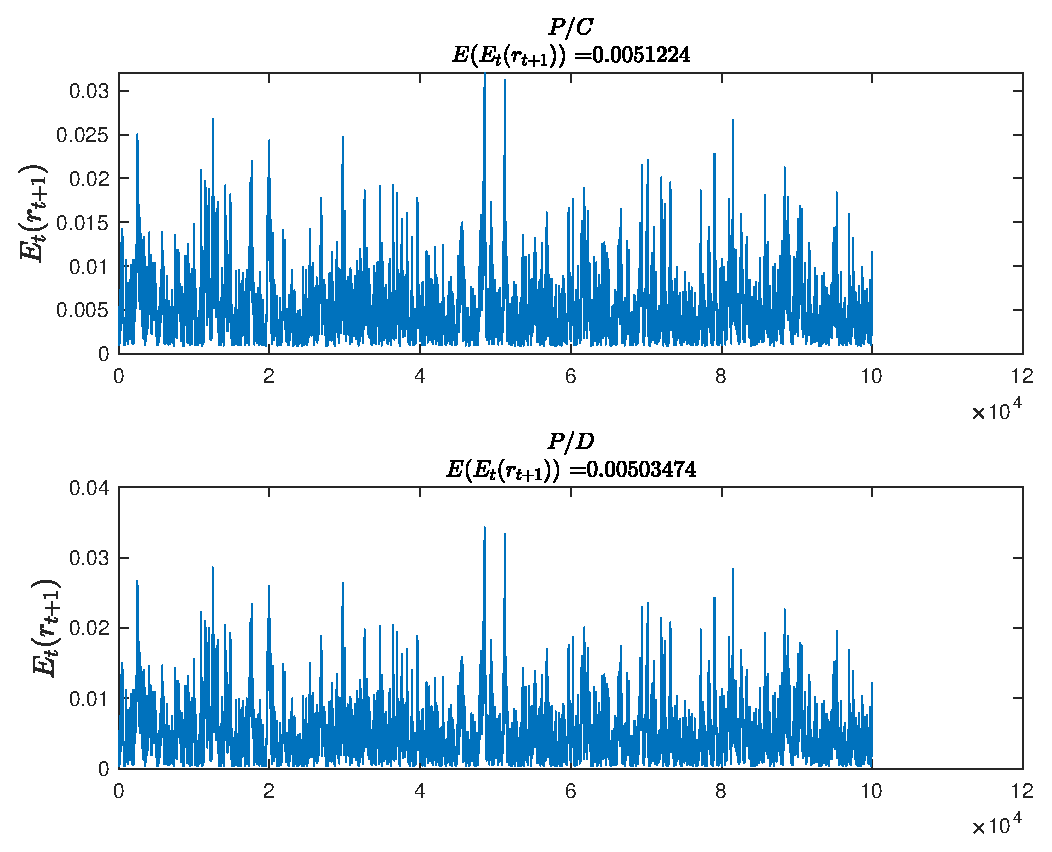
\includegraphics{Figures/Excess_Rets.eps}
    \label{fig:ExpExRets}
\end{figure}
This figure plots the true expected monthly returns of the model. That is for each $t\in\{1,2,...,100.000\}$ the model uses available information up until $t$ to determine the conditional future mean of returns before $t+1$ realizes. 

\begin{figure}[H]
    \centering
    \caption{Chain of simulated annual $P/D$, $P/C$}
    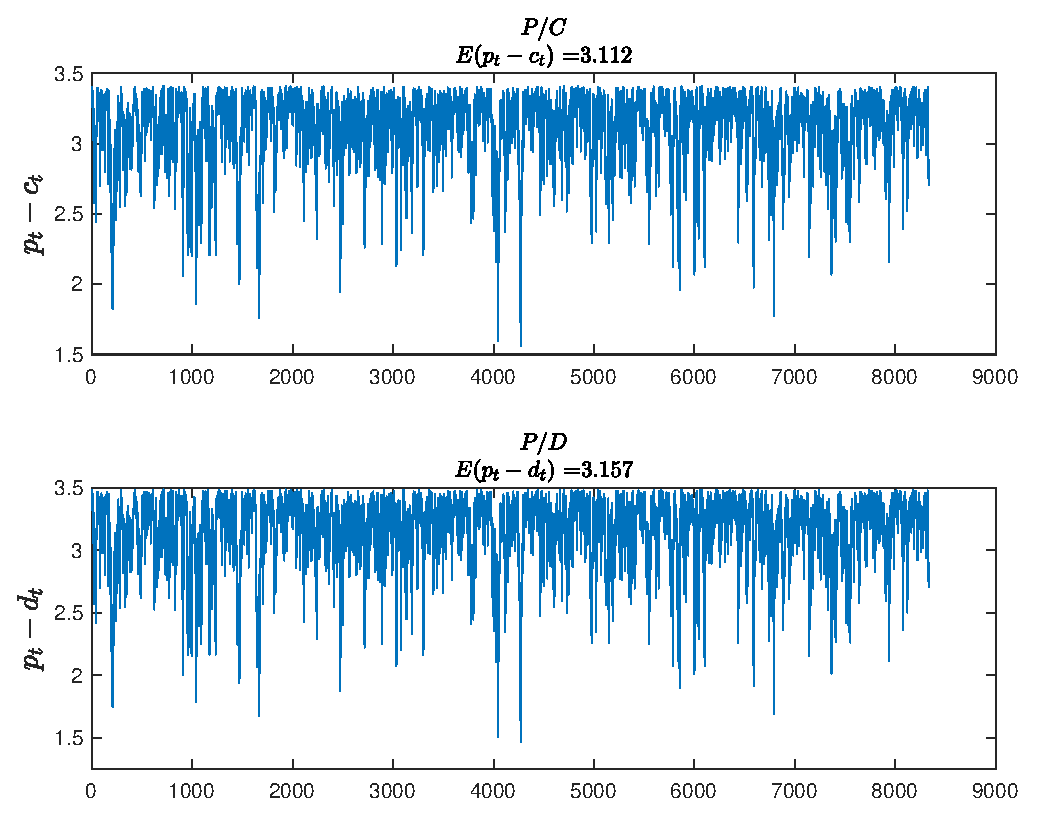
\includegraphics{Figures/PCPD_chain.eps}
    \label{fig:PCPD}
\end{figure}


\section{Code}
\subsection{Main Script and Regressions}
\label{sec:app1}
\lstinputlisting[language=Matlab]{Code_v2/MAIN.m}



\subsection{Functions called by main script}
\label{sec:app2}
\lstinputlisting[language=Matlab]{Code_v2/Functions/mkgrids.m}
\lstinputlisting[language=Matlab]{Code_v2/Functions/findlpc.m}
Note here that an additional file is required! Available here: \url{http://www.holoborodko.com/pavel/numerical-methods/numerical-integration/}\\
This is a \texttt{.mex} file calling a \texttt{c++}-function, greatly increasing the computational efficiency of the integration process. The built-in numerical integrator of \textsc{MatLab} can be used if preferred though.
\lstinputlisting[language=Matlab]{Code_v2/Functions/GaussLegendre.m}
\lstinputlisting[language=Matlab]{Code_v2/Functions/pdint.m}
\lstinputlisting[language=Matlab]{Code_v2/Functions/pdmotor.m}
\lstinputlisting[language=Matlab]{Code_v2/Functions/strans.m}
\lstinputlisting[language=Matlab]{Code_v2/Functions/interp.m}
\lstinputlisting[language=Matlab]{Code_v2/Functions/finders.m}
\lstinputlisting[language=Matlab]{Code_v2/Functions/intpcb.m}
\lstinputlisting[language=Matlab]{Code_v2/Functions/intemrs.m}
\lstinputlisting[language=Matlab]{Code_v2/Functions/mrsinsd.m}
\lstinputlisting[language=Matlab]{Code_v2/Functions/inter.m}
\lstinputlisting[language=Matlab]{Code_v2/Functions/erinsd.m}
\lstinputlisting[language=Matlab]{Code_v2/Functions/inter2.m}
\lstinputlisting[language=Matlab]{Code_v2/Functions/interd.m}
\lstinputlisting[language=Matlab]{Code_v2/Functions/erdinsd.m}
\lstinputlisting[language=Matlab]{Code_v2/Functions/inter2d.m}
\lstinputlisting[language=Matlab]{Code_v2/Functions/internorm.m}
\lstinputlisting[language=Matlab]{Code_v2/Functions/erd2ind.m}
\lstinputlisting[language=Matlab]{Code_v2/Functions/intelnr.m}
\lstinputlisting[language=Matlab]{Code_v2/Functions/intelnr2.m}
\lstinputlisting[language=Matlab]{Code_v2/Functions/intelnrcb.m}
\lstinputlisting[language=Matlab]{Code_v2/Functions/ercbin.m}
\lstinputlisting[language=Matlab]{Code_v2/Functions/annvars.m}
\lstinputlisting[language=Matlab]{Code_v2/Functions/chgfreq.m}
\lstinputlisting[language=Matlab]{Code_v2/Functions/simvars.m}
\lstinputlisting[language=Matlab]{Code_v2/Functions/simulacorr.m}
\lstinputlisting[language=Matlab]{Code_v2/Functions/lambda.m}
\lstinputlisting[language=Matlab]{Code_v2/Functions/lambda_Helper.m}
\lstinputlisting[language=Matlab]{Code_v2/Functions/selif.m}
\lstinputlisting[language=Matlab]{Code_v2/Functions/q_s.m}
\lstinputlisting[language=Matlab]{Code_v2/Functions/z_s.m}
\lstinputlisting[language=Matlab]{Code_v2/Functions/nwest.m}
\lstinputlisting[language=Matlab]{Code_v2/Tables/Table_Generator.m}
\lstinputlisting[language=Matlab]{Code_v2/Figures/Figures_CC1998.m}
\lstinputlisting[language=Matlab]{Code_v2/Calibration/Model_Calibration.m}
\begin{comment}
\end{comment}




\clearpage


\end{document}